In this case only two metrics are important for evaluation --- the cell area and the cell count (see Table \ref{table:gfp-metrics}). Both Pearson correlation and Spearman rank coefficients are lower than in previous experiments. Influence of additional segmentation of dead cells by the model lowers correlation scores, however they still signalize the presence of a strong correlation between prediction and ground truth. 
\begin{table}[H]
    \centering
    \caption{Correlation coefficients for practical biological evaluation}
        \begin{adjustbox}{width=0.4\textwidth}
            \begin{tabular}{|c|c|c|}\hline
                BCE loss&Pearson&Spearman
                \\\hline\hline
                Number of ER&0.67&0.64\\\hline
                Area&0.82&0.75\\\hline
            \end{tabular}
            \label{table:gfp-metrics}
        \end{adjustbox}
\end{table}

Violin and scattter plots depicting the two above mentioned metrics are shown in Figure \ref{fig:gfp-bce-metrics}.
\begin{figure}[H]
	\begin{center}
		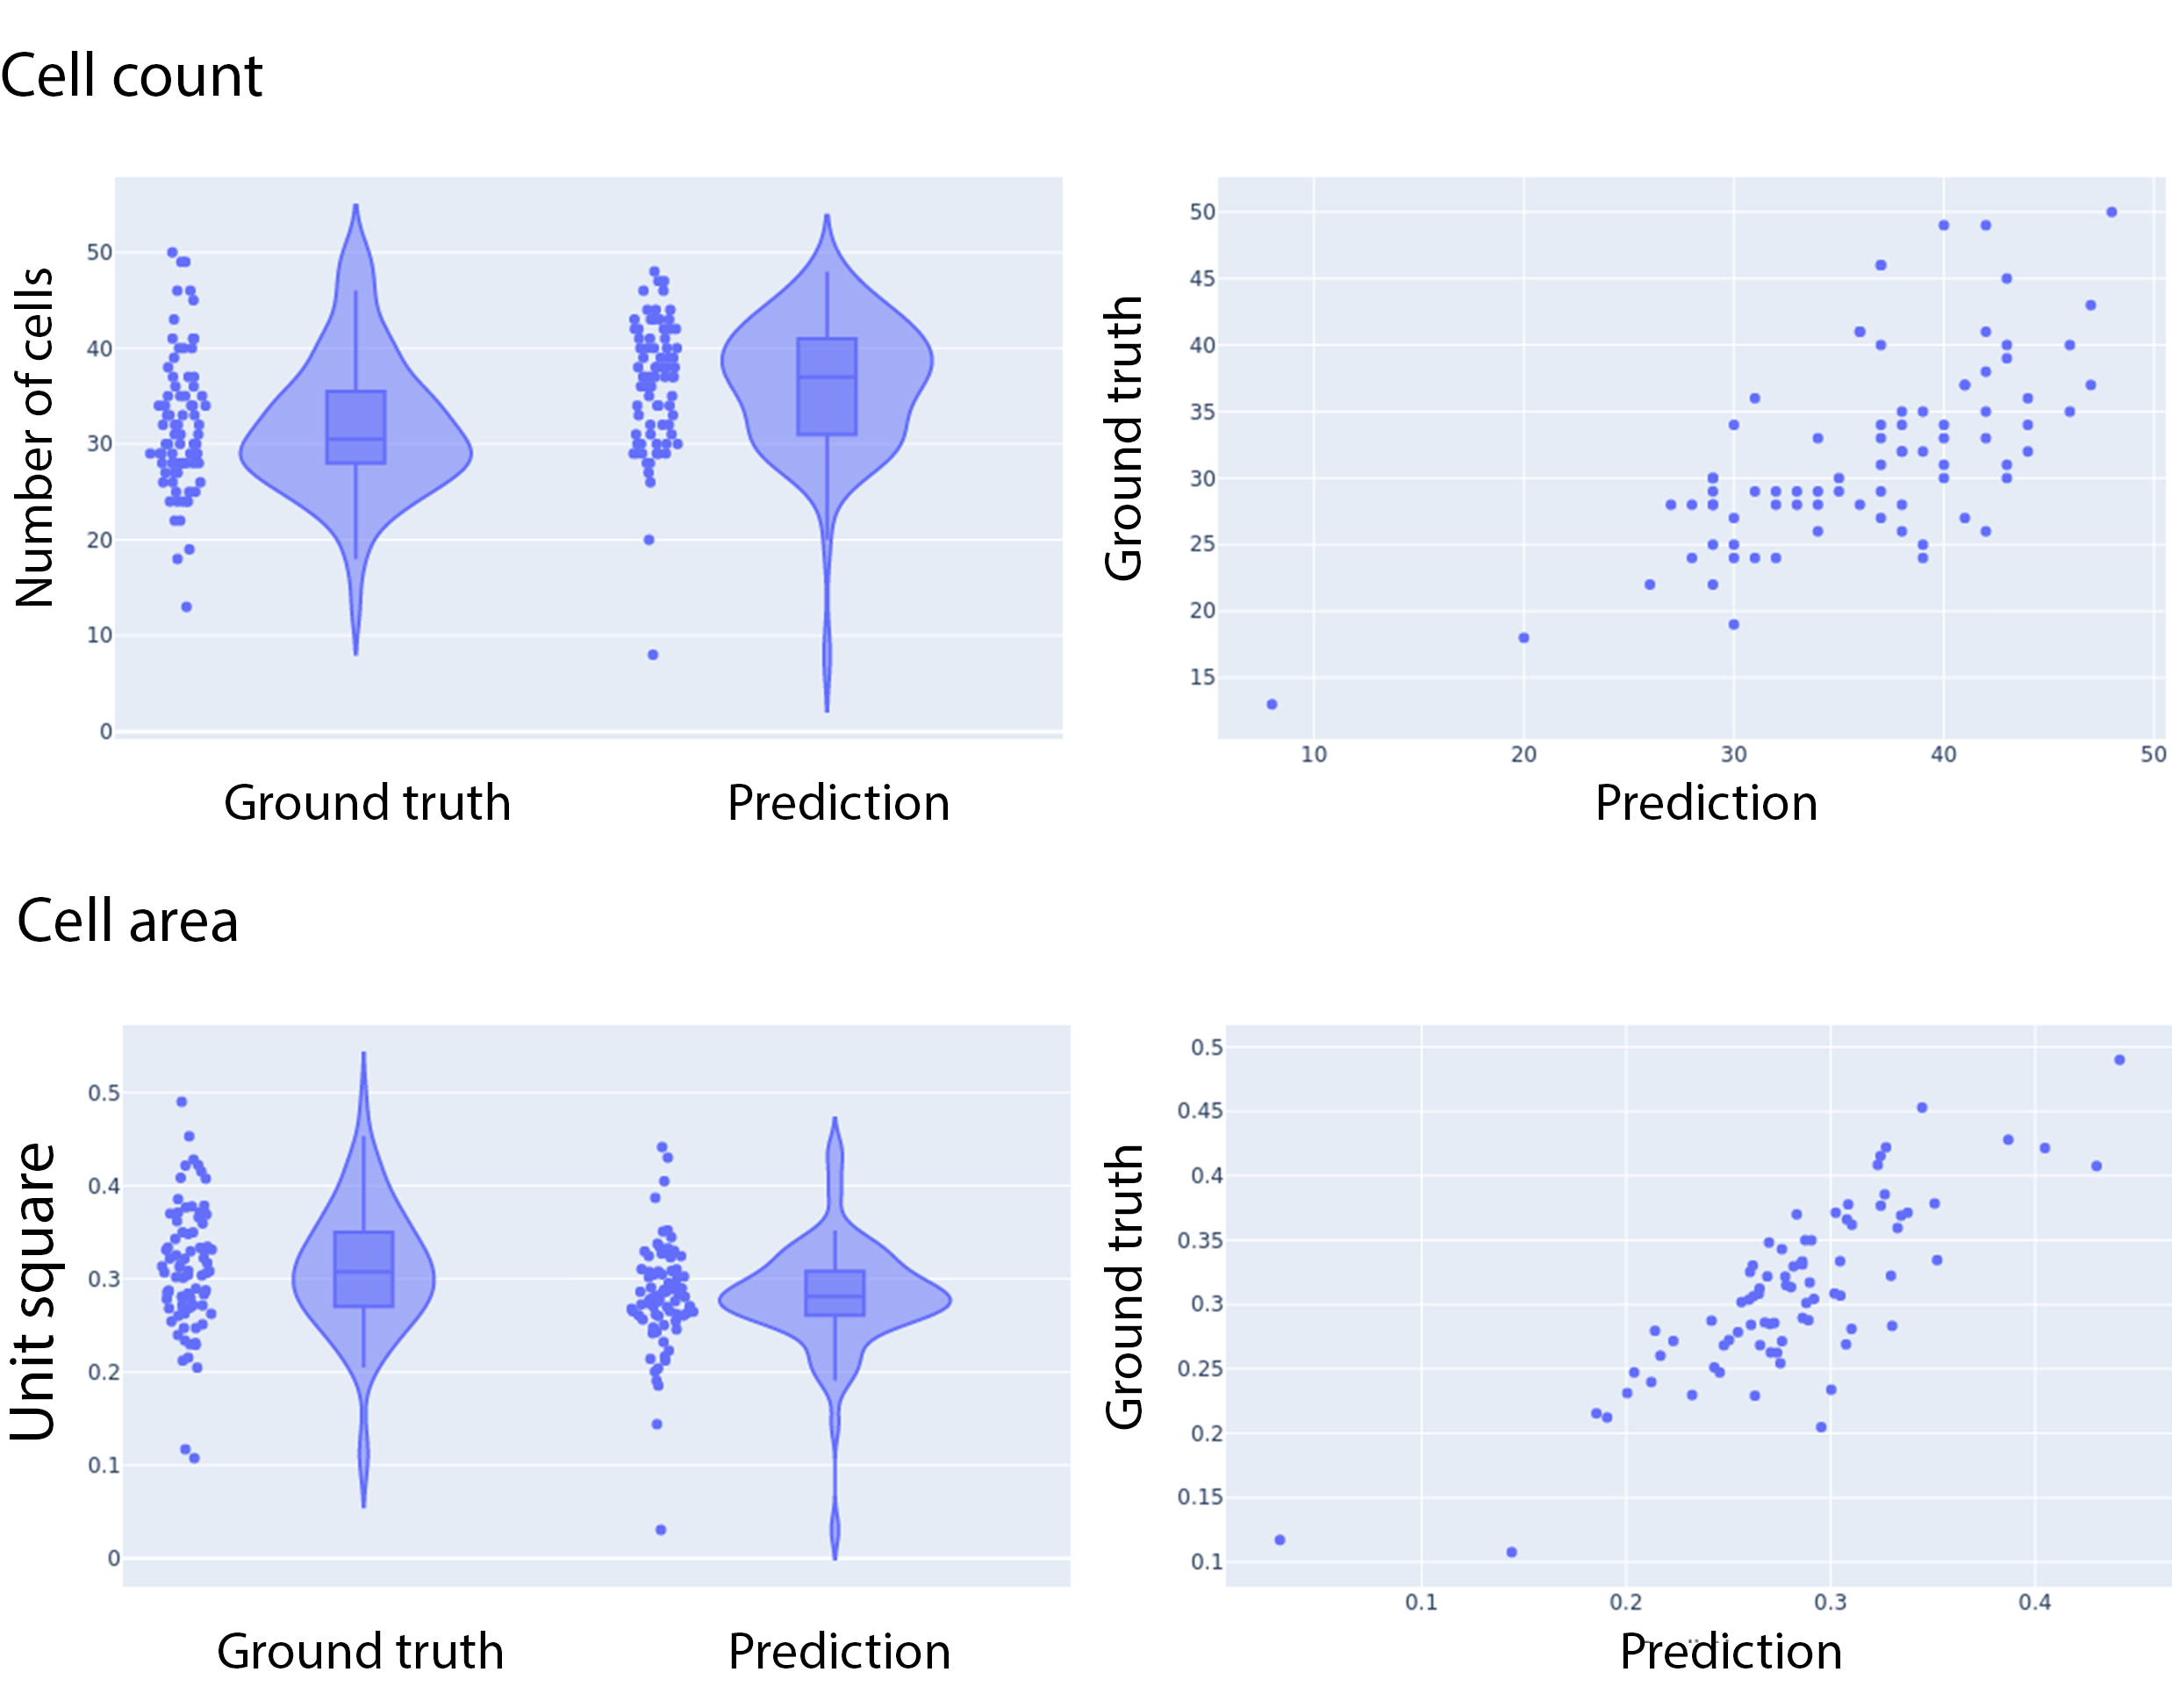
\includegraphics[width=\linewidth]{bilder/gfp/binary-bce/gfp-bce-metrics.png}
		\caption{Biological metrics}\label{fig:gfp-bce-metrics}
	\end{center}
\end{figure}